% modo presentación. si se cambia a modo notas se imprimen las notas (creo)
%\documentclass[xcolor={dvipsnames,x11names,svgnames},aspectratio=169,notes]{beamer}
% \mode<presentation>
%handout de las diapositivas, comentar arriva!
% handout de la presentacion
%\documentclass[handout,xcolor={dvipsnames,x11names,svgnames},aspectratio=169,notes]{beamer}
%\mode<handout>

% paquete beamer, opciones para nombres de colores y aspect ratio de panatalla grande.
%\documentclass[a4paper,12pt]{article}
%\usepackage{beamerarticle}

% para no tener problemas con acentos etc.
\usepackage[utf8]{inputenc}
% en español
\usepackage[spanish]{babel}
%matemática
\usepackage{amsmath}
% este no se si hace falta pero por las dudas
\usepackage{graphicx}
% para incluir peliculas
\usepackage{multimedia}
% para usar segunda pantalla
\usepackage{pgfpages}
\usepackage{pgf}
% para hacer dibujitos
\usepackage{tikz}
\usetikzlibrary[automata,calc,arrows,decorations.pathmorphing,backgrounds,shapes,
patterns,positioning,fit,petri,overlay-beamer-styles]
\tikzstyle{every picture}+=[remember picture]
%recuadros sencillos
%\usepackage{tcolorbox}
% enumeradores intercambiables
\usepackage{enumerate}
% para subtitulos en figuras
\usepackage{subcaption}
%listings for code input
\usepackage{listings}
%verbatim input from file!
\usepackage{verbatim}
\usepackage{fancyvrb}
% para modificar los encabezados y pies de página.
%\usepackage{fancyhdr}
%\pagestyle{fancy}
\usepackage{standalone}

\definecolor{codegreen}{rgb}{0,0.6,0}
\definecolor{codegray}{rgb}{0.5,0.5,0.5}
\definecolor{codepurple}{rgb}{0.58,0,0.82}
%\definecolor{backcolour}{rgb}{0.95,0.95,0.0.1}

\lstset{
    basicstyle=\fontsize{8}{10}\selectfont\ttfamily, 
    backgroundcolor=\color{Beige},   
    frame=lines,
    commentstyle=\color{codegreen},
    keywordstyle=\color{magenta},
    numberstyle=\tiny\color{codegray},
    stringstyle=\color{codepurple},
    breakatwhitespace=false,         
    breaklines=true,                 
    captionpos=b,                    
    keepspaces=true,                 
    numbers=left,                    
    numbersep=5pt,                  
    showspaces=false,                
    showstringspaces=false,
    showtabs=false,                  
    tabsize=4
}



% para mostrar las notas en modo presentacion. 
%\setbeameroption{show notes}
%para ocultar las notas
%\setbeameroption{hide notes}
%para dejar las notas en la segunda patnalla
%\setbeameroption{show notes on second screen}
%incluyo los paquetes necesarios

% en caso de handouts, ver 2 en 1 o 4 en 


% en forma arbitraria decid que los parrafos no llevan indentación.
\setlength{\parindent}{0cm}

% incluyo los beamercolors
%%%%%%%%%% BEAMERCOLORS
% el recuadro para el titulo
\setbeamercolor{title}{fg=white,bg=Purple}
% el recuadro para el subtitulo
\setbeamercolor{subtitle}{fg=white,bg=DarkOliveGreen}
% los títulos de las secciones tienen su colorinche:
\setbeamercolor{sectionbox}{fg=white,bg=Purple}
% cada diapositiva tendrá su color de título.
\setbeamercolor{frametitle}{fg=white,bg=ForestGreen}
% el título de las secciones tienen también su color. 
\setbeamercolor{sectiontitle}{fg=white,bg=violet}

%%%% CUSTOM BEAMERCOLORS
% estos cuadros los defino para ubicar al lector en los temas que se tratan
% son los cuadritos que aparecen arriba del título. 
\setbeamercolor{structure0}{fg=white,bg=gray}
\setbeamercolor{structure1}{fg=black,bg=DarkGray}
\setbeamercolor{structure2}{fg=black,bg=lightgray}
% defino un cuadro para usar en alguna oportunidad, creo que para titulos. 
\setbeamercolor{whitebox}{fg=black,bg=white}
% un cuadro para resaltar
\setbeamercolor{highlight1}{fg=black,bg=Gold}

% beamer colors for headers and etc.
\setbeamercolor{header1}{fg=white,bg=Blue}
\setbeamercolor{header2}{fg=black,bg=Red}
\setbeamercolor{header3}{fg=black,bg=ForestGreen}

%code block
\setbeamercolor{codeblock}{fg=Blue, bg=Beige}
\setbeamerfont{codeblock}{family=\ttfamily,size=\scriptsize}


%incluyo el tema y modificaciones
%%% BEAMER THEME
% el tema 'boxes' es igual al default pero permite definir boxes de estructura 
% a mano. 
\mode<presentation>{
  \usetheme{boxes}
  % los boxes que identifican lo que se esta leyendo
    % box de la izquierda: la materia (subtitulo)
    \addheadbox{structure2}{\quad \tiny \insertshortsubtitle}
  %  box del medio en cabecera, el titulo de la clase
    \addheadbox{structure0}{\quad \tiny  \inserttitle \quad } 
  % box en a la derecha , eltítulo de la sección. 
    \addheadbox{structure1}{\quad \tiny \insertsection}
}
% tema interno y de colores para las diapositivas normales. 
\useinnertheme{rectangles}
\usecolortheme{dove}
% la fuente de las ecuaciones
\usefonttheme[onlymath]{serif}

% entorno codeblock para meter piezas de código.
% el color se definió en BEAMERCOLORS

\newenvironment{codeblock}
{
  \begin{beamercolorbox}{codeblock}
    \usebeamerfont{codeblock}
}
{
  \end{beamercolorbox}
}



% modifico los temas
  \titlegraphic{%
\includegraphics[width=0.25\textwidth]{./PREAMBLE/logo-isabt25.png}
                
\includegraphics[width=0.25\textwidth]{./PREAMBLE/logo-isabato.png}
  		\hfill
		
\includegraphics[width=0.25\textwidth]{./PREAMBLE/ISOLOGOCNEA.png}
		\hfill
  		
\includegraphics[width=0.25\textwidth]{./PREAMBLE/unsam-horizontal.png}}

\mode<presentation>{
\setbeamertemplate{title page}[center]
{
  %
\includegraphics[width=0.25\textwidth]{./PREAMBLE/ISOLOGOCNEA.png}
  \inserttitle
  \insertsubtitle
  \insertauthor
  \insertinstitute
%  \inserttitlegraphic
}
}


% defino el template para las dapositivas con los titulos de las secciones. 
%es una recetita que saqué de algun lado. 
\setbeamertemplate{section page}{
  \begin{beamercolorbox}[ht=5ex,dp=1ex,wd=\paperwidth,center]{sectionbox}
    \begin{centering}
     \usebeamerfont{section  title} \insertsection 
    \end{centering}
  \end{beamercolorbox}
}
\AtBeginSection[]{
  \begin{frame}[plain]
    \begin{center}
    \quad \inserttitle \quad  
    \end{center}
    \sectionpage
  \end{frame}
}

% remover los simbolos de navegacion
% porque sacan espacio 
\mode<presentation>{
\setbeamertemplate{navigation symbols}{}
\setbeamertemplate{footline}[page number]
% me gustan los titulos a la derecha
\setbeamertemplate{frametitle}[default][right]%{
}
\mode<handout>{
 \setbeamertemplate{headline}{}
 \setbeamertemplate{frametitle}{}
 \setbeamertemplate{background}{
   \tikz\node [rectangle,minimum width=0.995\paperwidth,
   minimum height=0.995\paperheight,draw,anchor=south west,
   line width=2pt]  {};
 }
 \setbeamertemplate{footline}{}
}
% aparentemente el siguiente beamertemplate
%se ejecuta en modo artículo. habría que ver
%la forma de sacale probecho. 
% notar que vale solo para las framesque se incluyen 
% directamente en el artículo y no vale para 
% \includeslide.
% \setbeamertemplate{frame begin}
% \setbeamertemplate{frame end}


% no se si es el mejor lugar para definirlo, 
% pero las \includeslides deben quedar fijas al
% tamaño de la página:

%\mode<article>{
%\renewcommand\includeslide[1]{
%  \includeslide[width=\textwidth]{#1}
%}
%}


% defino el template para la diapositiva del título

%%%%%%%%%%%%%%%%%%%%%%%%%%%%%%%%
% Defino la presentación
%%%%%%%%%%%%%%%%%%%%%%%%%%%%%%%%
\title{
  \mode<article>{

\includegraphics[height=1cm]{./PREAMBLE/logo-isabt25.png}
\hfill

\includegraphics[height=1cm]{./PREAMBLE/ISOLOGOCNEA.png}
\hfill
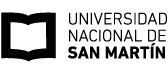
\includegraphics[height=1cm]{./PREAMBLE/logo-unsam.png}
\\} Solucion de Sistemas Lineales Mixtos}
\subtitle[Modelización 2019]{ Modelización de Propiedades y Procesos 2019 }
\author{Ruben Weht\inst{1}\inst{2} \and Mariano Forti\inst{1}\inst{3} }
\institute{
  \inst{1}Instituto de Tecnología Prof. Jorge Sabato
  \and
  \inst{2}Fisica del Sólido, Edificio TANDAR, \url{weht@cnea.gov.ar},
  interno 7104
  \and
  \inst{3}División Aleaciones Especiales, Edificio 47 (microscopía),
  \url{mforti@cnea.gov.ar}, interno 7832
}
\subject{Solucion de Problemas Lineales Mixtos}
\keywords{Elementos Finitos, Sistemas Mixtos}
\date{2020}

% Inicia el documento.
\begin{document}
% Título de la clase. 
\mode<presentation>{
\begin{frame}[plain]
\titlepage
\end{frame}
}
\mode<article>{
  \maketitle
}

\section{Ejemplo: Problema de los Resortes}
\mode<article>

Consideremos el problema 1 de la guía, en el que una cadena de tres resortes, empotrada en el
extremo izquierdo, es solicitada por un desplazamiento en el extremo derecho.

Las condiciones sobre los extremos nombradas anteriormente nos dan las condiciones de contorno
sobre la cadena de resortes.

Para poder resolver la fuerza necesaria para efectuar el desplazamiento usando el método de
elementos finitos, dividimos el problema de forma natural en tres elementos. Cada resorte será un
elemento, y cada elemento tendrá dos nodos, de modo que todos los grados de libertad del problema
pueden representarse en cuatro nodos. Cada nodo marca un extremo de un resorte. 

Los numeremos los Elementos de 1 a 3 indicados con cajas en la figura, y los nodos de 1 a 4.
indicados con círculos en la Figura \ref{FiguraNumeracionGL}

\mode*

\begin{frame}[label=FrameNumeracionGL]
  \frametitle<presentation>{Problema de los Resortes}

  \begin{figure}
    \includegraphics[width=\textwidth,page=2, trim=5cm 7cm 5cm 8cm, clip=true]
    {./Libreoffice/MEF01_2018.pdf}
    \mode<article>{
      \caption { Esquema del problema \protect\label{FiguraNumeracionGL} }
    }
  \end{figure}


\end{frame}

\mode<all>

\mode<article>


Consideremos las fuerzas que cada Elemento o resorte ejerce sobre los nodos, tal cual se hizo en
la clase teórica. Agreguemos ahora un poco de detalle sobre cada uno de los resortes.

\mode*

\mode<all>
 

\subsection{Fuerzas en los Nodos}
\subsubsection{Fuerzas sobre el elemento 1}

\mode<article>

Como se ilustra en la Figura \ref{FigureFuerzasElemento1} Las fuerza sobre el nodo 1 del Elemento
1 es $f_1^1$ , mientras que la fuerza sobre el nodo 2 del Elemento 1 es $f_2^1$. Ambas fuerzas
son de igual módulo pero opuestas, y quedan determinadas por el estiramiento del resorte. Este
estiramiento será directamente la diferencia de corrimientos entre los nodos que determinan el
elemento 1 y 2. Si las posiciones de dichos nodos son $x_1$ y $x_2$, se pueden escribir las
fuerzas como en la ecuación (\ref{EqElemento1}). 

Notar que ha quedado definida la matriz de rigidez elemental del 
Elemento 1, $\mathbf{k_1 ^{el} }$.

\mode*

\begin{frame}[label=FrameFuerzasElemento1]
  \frametitle<presentation>{Fuerzas sobre el Elemento 1}

  \begin{figure}
    \includegraphics[width=\textwidth,page=3, trim=5cm 8cm 5cm 6cm, clip=true]
    {./Libreoffice/MEF01_2018.pdf}
    \mode<article>{
      \caption{\protect\label{FigureFuerzasElemento1} Fuerzas sobre el elemento 1}
    }
  \end{figure}

  \begin{equation} 
    \label{EqElemento1}
    \begin{split}
      f_1^1 &= -k_1 (x_2 - x_1)\\[10pt]
      f_2^1 &= k_1 (x_2 - x_1)
    \end{split}
    \quad \Rightarrow \quad
     \begin{pmatrix}
       f_1^1\\[10pt]
       f_2^1
     \end{pmatrix}
     =
     \underbrace{
       k_1 
       \begin{pmatrix}
	 1 & -1 \\[10pt]
	 -1 & 1 
       \end{pmatrix}
     }_{ \mathbf{ k_1 ^{el} } }
    \begin{pmatrix}
      x_1 \\[10pt]
      x_2
    \end{pmatrix}
%    
  \end{equation}
          
\end{frame}

\mode<all>


\begin{frame}[label=FrameFuerzasElemento2]
  \frametitle<presentation>{Fuerzas sobre el Elemento 2}

  \begin{figure}
    \includegraphics[width=\textwidth,page=4, trim=5cm 8cm 5cm 6cm, clip=true]
    {./Libreoffice/MEF01_2018.pdf}
    \mode<article>{
      \caption{\protect\label{FigureFuerzasElemento2} Fuerzas sobre el elemento 2}
    }
  \end{figure}

  \begin{equation} 
    \label{EqElemento2}
    \begin{split}
      f_1^2 &= -k_2 (x_3 - x_2)\\[10pt]
      f_2^2 &= k_2 (x_3 - x_2)
    \end{split}
    \quad \Rightarrow \quad
     \begin{pmatrix}
       f_1^2\\[10pt]
       f_2^2
     \end{pmatrix}
     =
     \underbrace{
       k_2 
       \begin{pmatrix}
	 1 & -1 \\[10pt]
	 -1 & 1 
       \end{pmatrix}
     }_{ \mathbf{ k_2 ^{el} } }
    \begin{pmatrix}
      x_2 \\[10pt]
      x_3
    \end{pmatrix}
%    
  \end{equation}
          
\end{frame}



\subsubsection{Fuerzas sobre el elemento 3}

\mode<article>

Por útlimo, para el Elemento 3 el estiramiento queda determinado por los nodos 4 y 3, de manera
que los grados de libertad relevantes son $x_3$ y $x_4$

\mode*


\begin{frame}[label=FrameFuerzasElemento3]
  \frametitle<presentation>{Fuerzas sobre el Elemento 3}

  \begin{figure}
    \includegraphics[width=\textwidth,page=5, trim=5cm 8cm 5cm 6cm, clip=true]
    {./Libreoffice/MEF01_2018.pdf}
    \mode<article>{
      \caption{\protect\label{FigureFuerzasElemento3} Fuerzas sobre el elemento 3}
    }
  \end{figure}

  \begin{equation} 
    \label{EqElemento2}
    \begin{split}
      f_1^3 &= -k_3 (x_4 - x_3)\\[10pt]
      f_2^3 &= k_3 (x_4 - x_3)
    \end{split}
    \quad \Rightarrow \quad
     \begin{pmatrix}
       f_1^2\\[10pt]
       f_2^2
     \end{pmatrix}
     =
     \underbrace{
       k_3 
       \begin{pmatrix}
	 1 & -1 \\[10pt]
	 -1 & 1 
       \end{pmatrix}
     }_{ \mathbf{ k_3 ^{el} } }
    \begin{pmatrix}
      x_3 \\[10pt]
      x_4
    \end{pmatrix}
%    
  \end{equation}
          
\end{frame}

\mode<all>


\subsection{Fuerzas Globales}

\mode<article>

La fuerza total sobre cada uno de los nodos es la suma de todas las fuerzas que actúa sobre cada
uno de ellos. Al escribir estas ecuaciones globales, es posible acoplar a todos los grados de
libertad a partir de las ecuaciones locales, expandiendo cada una de ellas de manera que
aparezcan en forma explícita todos los grados de libertad del problema $x_1$, $x_2$, $x_3$ y
$x_4$. La fuerza global sobre cada nodo puede numerarse $F_1$, $F_2$, $F_3$ y $F_4$ .

\mode*

\begin{frame}[label=FrameFuerzasGlobales]
  \frametitle<presentation>{Fuerzas Globales}

  \begin{figure}
    \fbox{
    \includegraphics[width=\textwidth,page=6, trim=5cm 11cm 3cm 7cm, clip=true]
    {./Libreoffice/MEF01_2018.pdf}
  }
    \mode<article>{
      \caption{\protect\label{FigureFuerzasGlobales} Fuerzas Globales}
    }
  \end{figure}
%
 \tiny 
  \begin{equation}\label{EqSistemaLinealExpandido}
    \begin{aligned}
      F_1 &= f_1^1  = -k_1( x_2-x_1) =
                   x_1 (k_1) + x_2(-k_1)+ x_3(0) + x_4(0)\\
      F_2 &= f_1^2 + f_2^1 = k_1( x_2-x_1) -k_2(x_3 - x_2) = 
                   x_1 (-k_1) + x_2(k_1+k_2)+ x_3(-k_2) + x_4(0)\\
      F_3 &= f_2^2 + f_1^3 = k_2( x_3-x_2) - k_3 (x_4 - x_3) = 
                    x_1 (0) + x_2(-k_2)+ x_3(k_2 + k_3) + x_4(-k_3)\\
      F_4 &= f_2^3 = k_3( x_4-x_3)=
                     x_1 (0) + x_2(0)+ x_3(-k_3) + x_4(k_3)
    \end{aligned}
  \end{equation}
%
\end{frame}

\mode<article>

Este sistema de ecuaciones puede pensarse en forma Lineal, donde tenemos un
vector de Fuerzas $\mathbf{F}$  y un vector de desplazamientos $\mathbf{x}$. Notar que también
queda definida la matriz de rigidez global delsistema $\mathbf{M}$

El problema del  sistema lineal de la ecuación (\ref{eqSistemaLineal})
es que por las condiciones de contorno
planteadas al principio, las incógnitas y las condiciones de contorno están
repartidas en forma arbitraria entre el vector de desplazamientos y el vector
de fuerzas. Por lo tanto, es necesario extender algo de nuestro desarrollo.


\mode*

\begin{frame}<1>[label=FrameMatrizRigidez]
  \frametitle<presentation>{Matriz de Rigidez Global}
  \frametitle<2->{Separación del Sistema Lineal}

  \begin{equation} \label{eqSistemaLineal}
    \onslide<1> \underbrace{
      \onslide<1->
      \begin{pmatrix}
	k_1  & -k_1     & 0    & 0 \\
	-k_1 & k_1 +k_2 & -k_2 & 0 \\
	0    & -k_2     & k_2 + k_3 & -k3\\
	0    &  0       & -k_3      & k_3
      \end{pmatrix}
    \onslide<1> }_{\mathbf{M}}
  \onslide<1->
    \begin{pmatrix}
      x_1\\
      x_2\\
      x_3\\
      x_4
    \end{pmatrix}
    =
    \begin{pmatrix}
      F_1\\
      F_2\\
      F_3\\
      F_4
    \end{pmatrix}
  \end{equation}

  \only<1>{
  \mode<presentation>{
    \begin{columns}
      \column{0.5\textwidth}

      $x_i$ : desplazamiento del nodo $i$

      $F_i$ : fuerza en el nodo $i$

      \column{0.5\textwidth}

      Vínculos: $x_1$, $x_4$

      Fuerzas conocidas: $F_2$, $F_3$

    \end{columns}
  }

}
\onslide<3->
\tikz[overlay] \draw[->,draw]  (0,2.5) -- 
  (1,2.5);
\tikz[overlay]
  \draw[opacity=0.5,fill=blue] (1.5,2.4)
  rectangle (2.2, 2.6) ;
\onslide<4->
\tikz[overlay] \draw[->,draw]  (0,2) -- 
  (1,2);
\end{frame}

\mode<all>
	

\section{Solucion de sistemas lineales mixtos}

\mode<article>

Recordemos las condiciones de contorno. El nodo 1 se encuentra empotrado por lo
que su desplazamiento está fijo en $x_1=0$. El nodo 4 está obligado a
desplazarse $x_4 = \delta$ de su posición de equilibrio.  La fuerza necesaria
para que estos dos nodos permanezcan en esas condiciones, $F_1$ y $F_4$ son
desconocidas. 

Por otro lado, los nodos 2 y 3 se han desplazado una cantidad desconocida, pero
como suponemos que están en equilibrio estático podemos decir que no hay
fuerzas externas aplicadas en ellos, $F_2 = F_3 = 0$.

En principio, el sistema lineal encontrado representa un sistema de ecuaciones.
Tratemos primero las ecuaciones que corresponden con los desplazamientos
desconocidos $x_2$ y $x_3$ en el ejemplo del resorte. La operatoria consiste en
expandir las ecuaciones correspondientes en todos los grados de libertad, tal y
como aparecen en la ecuación \ref{EqSistemaLinealExpandido}.

Luego deben ser reordenados los términos de los grados de libertad vinculados
$x_1$ y $x_4$ a la derecha del igual, de manera de dejar del lado izquierdo del
igual solo a los términos de los grados de libertad incógnita $x_2$ y $x_3$, 

\mode*

\begin{frame}<presentation>[label=FrameSeparacionSistema]
  \frametitle{Separación del sistema lineal}

  \begin{tikzpicture}[
      overlay,remember picture,
      inc/.style={fill=red, opacity=0.2},
      vin/.style={fill=blue, opacity=0.2}
    ]
    \coordinate (O) at (1,0);
    \coordinate (E) at (10,-4);
    \coordinate (L1) at (1,0.5);
    \coordinate (L2) at (3,0.5);
    \coordinate (A) at (1.5,-1 );
    \coordinate (B) at (2.5,-1);
    \coordinate (C) at (5.5, -1);
    % las coordenadas de xvin y xinc
    \coordinate (X4) at (7,-2);
    \coordinate (X1) at (7,-0.5);
    \coordinate (X3) at ($(X4)+(0,0.5)$);
    \coordinate (F3) at (8.5,-1.5);
    \coordinate (F2) at ($(F3)+(0,0.5)$);
    \coordinate (LI) at (1,1);
   % esta es el desplazamiento para el renglon de abajo 
    \coordinate (D) at (0,-0.5); 
    % este grid lo tengo que sacar despues
    \draw[gray] (O)  grid (E);
    \onslide<2->
    \draw[vin] (X4) rectangle ($(X4)+(L1)$);
    \draw[vin] (X1) rectangle ($(X1)+(L1)$);
    \draw[inc] (X3) rectangle ($(X3)+(LI)$);
    \onslide<2>
    \draw[vin] (A)         rectangle ($(A)+(L1)$);
    \draw[inc] (B)         rectangle ($(B)+(L2)$); 
    \draw[vin] (C)         rectangle ($(C)+(L1)$);
    \draw[vin] (F2) rectangle ($(F2)+(L1)$);
    \onslide<3>
    \draw[vin] ($(D)+(A)$) rectangle ($(A)+(L1)+(D)$);
    \draw[inc]  ($(D)+(B)$) rectangle ($(B)+(L2)+(D)$); 
    \draw[vin] ($(D)+(C)$) rectangle ($(C)+(L1)+(D)$);
    \draw[vin] (F3) rectangle ($(F3)+(L1)$);
    
  \end{tikzpicture}
  \begin{equation} \label{eqSistemaLineal}
    \matriz \vectorx  =  \vectorF
  \end{equation}

\onslide<2->{
\begin{equation}\begin{aligned}
    \ecuaciona \\ 
  \onslide<3->{ \ecuacionb }
\end{aligned}\end{equation}
}
\end{frame}

\begin{frame}[label=FrameReordenarEcuaciones23]
  \frametitle<presentation>{Reordenando Ecuaciones Para Incógnitas}
\begin{equation}  \label{EqReordenoIncognitas}
    \begin{aligned}
      \ecuaciona \\
      \ecuacionb \\
      \quad \Rightarrow \quad & \\
      \ecuacionao \\
      \ecuacionbo
    \end{aligned}
\end{equation}

\end{frame}

\mode<article>

Finalmente, pensemos en un vector de incógnitas $X_r = (x_2, x_3)$   y un
vector de vínculos $X_s  = (x_1, x_4)$ . Con estas definiciones, las
ecuaciones (\ref{EqReordenoIncognitas})  puede escribirse en forma matricial, de manera que
  quedarán definidas la \textbf{matriz de rigidez reducida} $\mathbf{K_{red} }$ 
  y la \textbf{matriz de coeficientes vínculos} $\mathbf{K_{vin}}$

\mode*

  \begin{frame}<1>[label=FrameSistemaReducido]
    \frametitle<presentation>{Reducción del Sistema}
    \begin{equation}\label{EqSistemaReducido}
      \underbrace{
	\begin{pmatrix} k_1 + k_2 & - k_2 \\ -k_2 & k_1 + k_2 \end{pmatrix}
	}_{ \mathbf{K_{red} } }
	\begin{pmatrix}x_2 \\ x_3\end{pmatrix}
	  = 
	  \begin{pmatrix}F_2 \\ F_3\end{pmatrix}
	    -
	  \underbrace{
	      \begin{pmatrix} -k_1 & 0 \\ 0 & -k1 \end{pmatrix}
	   }_{ \mathbf{ K_{vin} } }
	\begin{pmatrix}x_1 \\ x_4\end{pmatrix}
    \end{equation}

  \end{frame}


\mode<all>


\end{document}
